\section{1184013 - Helmi Azhar}
\subsection{Teori}
\begin{enumerate}

	\item Definisi Kecerdasan Buatan
	\hfill\break
	Kecerdasan Buatan atau Artifical Inteligence adalah suatu alat atau aplikasi yang diprogram memiliki suatu kemampuan yang dimiliki oleh manusia hal ini bertujuan agar suatu produk tersebut dapat berperilaku seperti manusia.

	\item Sejarah dan Perkembangan
	\hfill\break
Pada tahun 1959 pria bernama McCarthy merancang sebuah produk yang dapat memecahkan masalah. Pada awalnya seorang mahasiswa membuat program kecerdasan buatan yang dinamakan Geometry Theorm Prover yang digunakan untuk menjawab pertanyaan-pertanyaan yang ada. namun pada tahun 1960-1970 kecerdasan buatan ini kurang berkembang karena kurangnya wawasan untuk berkembang pada saat itu. Pada tahun 1980 kecerdasan buatan mulai berkembang kembali oleh Digital Equipment Corporation (DEC) yang menemukan sistem konfigurasi pada komputer baru hal ini masih berkembang sampai saat ini.

	\item Kecerdasan buatan terbagi atas beberapa metode yaitu:
	\hfill\break
	Supervised learning,  Klasifikasi, Regresi,Unsupervised Learning, Dataset, Trainingset dan juga Testingset.
	\begin{itemize}
		\item Supervised Learning
		\hfill\break
	Supervised Learning	adalah algoritma yang memiliki atribut khusus seperti x dan y untuk memprediksi.
		\item Klasifikasi
		\hfill\break
		Klasifikasi merupakan sampel yang dimiliki oleh dua atau lebih class yang dihimpun berdasarkan tingkat kemiripan ataupun jarak 
		\item Regresi
		\hfill\break
Regresi	merupakan suatu prediksi dimana apabila suatu hasil atau output yang diinginkan terdiri dari satu atau lebih variable contionous.
		\item Unsupervised Learning 
		\hfill\break
Unsupervised Learning  adalah algoritma yang tidak memiliki atribut tambahan yang akan diprediksi
		\item Data set
		\hfill\break
Data set	merupakan kondisi dimana hanya terdapat inputan data tanpa memiliki viariasi output yang sesuai
		\item Training Set
		\hfill\break
	Training Set	merupakan bagian dari data set yang digunakan untuk mempelajari beberapa properti		
		\item Testing Set
		\hfill\break
Testing Set	merupakan bagian data set yang digunakan untuk pengujian dari sebuah properti yang dipelajari
	\end{itemize}
\end{enumerate}
\subsection{Praktek}
\begin{enumerate}
	\item Instalasi Library scikit dari Anaconda, mencoba kompilasi dan uji coba ambil contoh kode dan lihat variabel explorer
	\hfill\break
	\begin{figure}[h]
		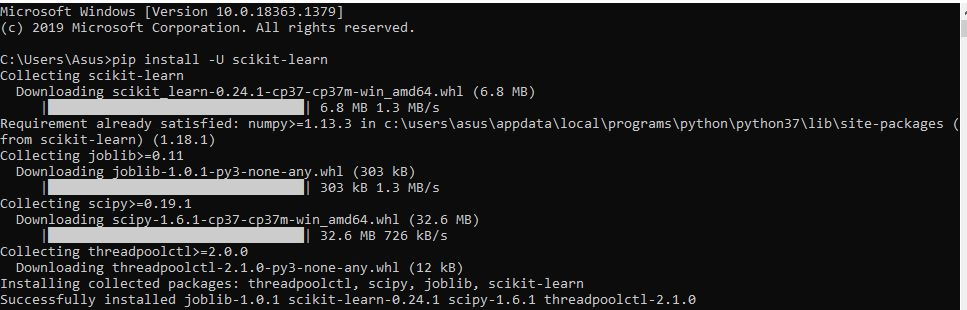
\includegraphics[width=10cm]{figures/1184013/chapter 1/01.JPG}
		\centering
		\caption{Instalasi Library Scikit Learn}
	\end{figure}
	\newpage\item Uji coba loading an example dataset
	\hfill\break
\lstinputlisting[firstline=7, lastline=16]{src/1184013/chapter1/tugas1.py}
\item Uji coba Learning dan predicting
	\hfill\break
	\lstinputlisting[firstline=17, lastline=32]{src/1184013/chapter1/tugas1.py}
\item Uji coba Model Persistence
	\hfill\break
	\lstinputlisting[firstline=35, lastline=63]{src/1184013/chapter1/tugas1.py}
	\item Uji coba Conventions
	\hfill\break
	\lstinputlisting[firstline=64, lastline=82]{src/1184013/chapter1/tugas1.py}
	\end{enumerate}
	\subsection{Penanganan Error}
\begin{enumerate}
	\item Screenshoot Error
	\begin{figure}[h]
		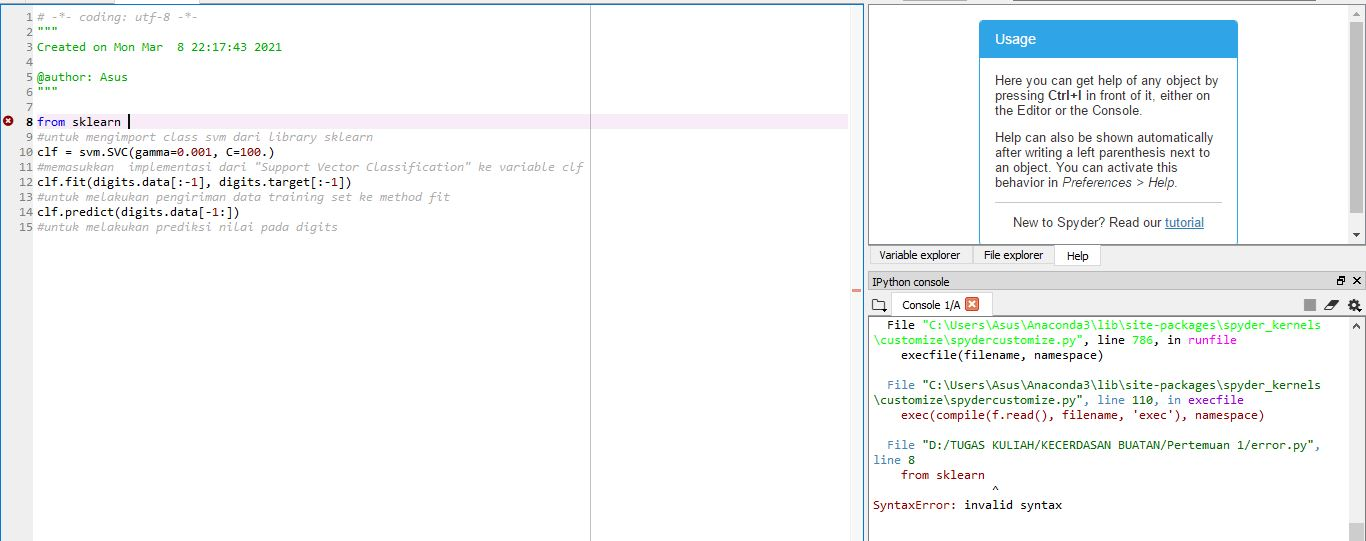
\includegraphics[width=10cm]{figures/1184013/chapter 1/eror.JPG}
		\centering
		\caption{Name Error}
	\end{figure}
	\newpage\item Tuliskan Kode Error dan Jenis Error
	\hfill\break
	\lstinputlisting[firstline=83, lastline=91]{src/1184013/chapter1/tugas1.py}
\hfill\break
	\item Cara Penangan Error
\hfill\break Tambahkan class svm agar kode program dapat terbaca
	\end{enumerate}
	\subsection{Bukti Tidak Plagiat}
\begin{figure}[h]
	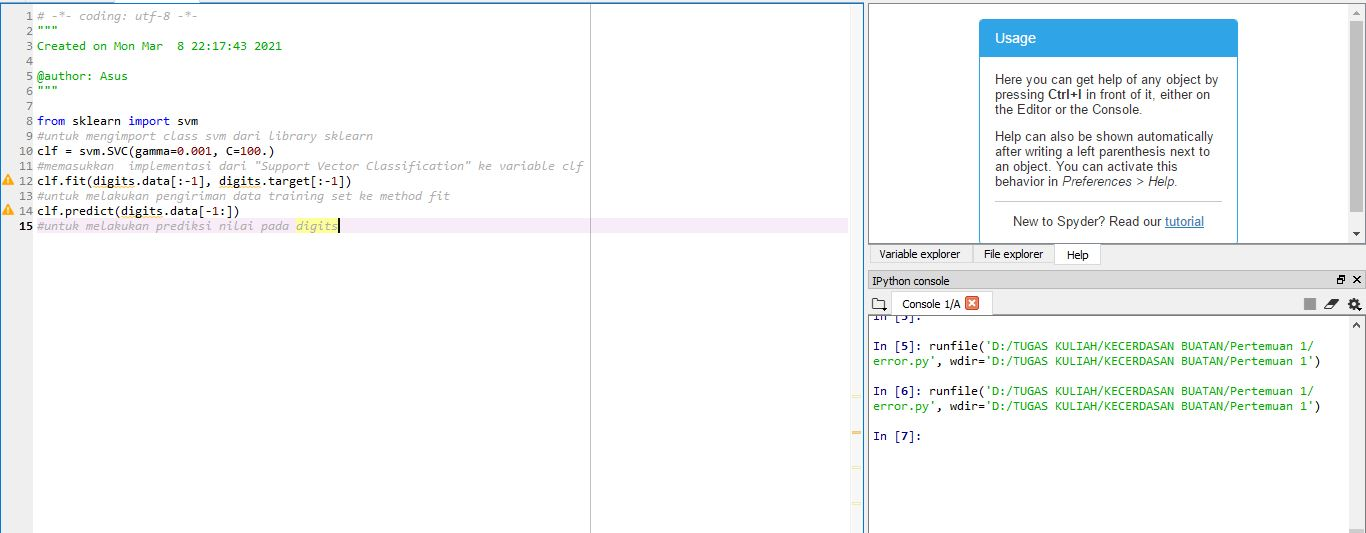
\includegraphics[width=10cm]{figures/1184013/chapter 1/error.JPG}
	\centering
	\caption{Bukti Tidak Melakukan Plagiat Chapter 1}
\end{figure}